\documentclass[mathserif]{beamer}
\usepackage[utf8]{inputenc}
\usepackage{amsmath}
\usepackage{amsfonts}
\usepackage{amssymb}
\usepackage{arydshln}
\usepackage{graphicx}
\usepackage{float}
\usepackage{picture}
\usepackage{dcolumn}
\usepackage{textpos}
 
%Information to be included in the title page:
\title{Embedded Software Design}
\author{Thomas S. Christensen}
\institute{University of Southern Denmark}
\date{Jan, 2017} 
 
\setbeamercolor{structure}{fg=grey}
\usetheme{metropolis}
\addtobeamertemplate{frametitle}{}{%
\begin{textblock*}{200mm}(\textwidth-1.5cm,-0.8cm)

\includegraphics[scale=0.15]{sdu_logo}
\end{textblock*}}

\begin{document}
 
\begin{frame}
	\section{Disposition}
	\frametitle{Embedded Software Design}
	Temperature Regulation\\
	\vfill
	Disposition:
	\begin{itemize}
		\item \textbf{Application}
		\item \textbf{System Overview}
		\item \textbf{DHT11}
		\item \textbf{Temperature Scaling}
		\item \textbf{PWM Generation}
	\end{itemize}
\end{frame}

\note{Jeg har lavet et lille projekt omkring temperatur regulering som jeg vil starte med at fortælle jer lidt om idag.
Først og fremmest vil jeg fortælle hvad præmissen er for systemet, så vil jeg give et lille overblik over systemet.
Herefter vil jeg snakke lidt om den primære del nemlig temperatur sensoren, hvordan kommunikationen med den foregår, og hvordan jeg implementerede driveren til den.
Så har jeg kort lidt om hvordan temperaturen bliver skaleret til at give en duty cycle og til sidst, et overblik over modulet der genererer PWM.}

\begin{frame}
	\section{Application}
	\frametitle{Application}
	\begin{columns}
		\begin{column}{.49\linewidth}
			\centering
			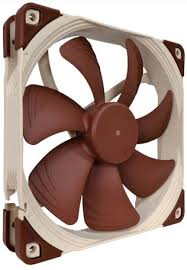
\includegraphics[width=.5\linewidth]{graphics/fan.jpg}
		\end{column}
		\begin{column}{.49\linewidth}
			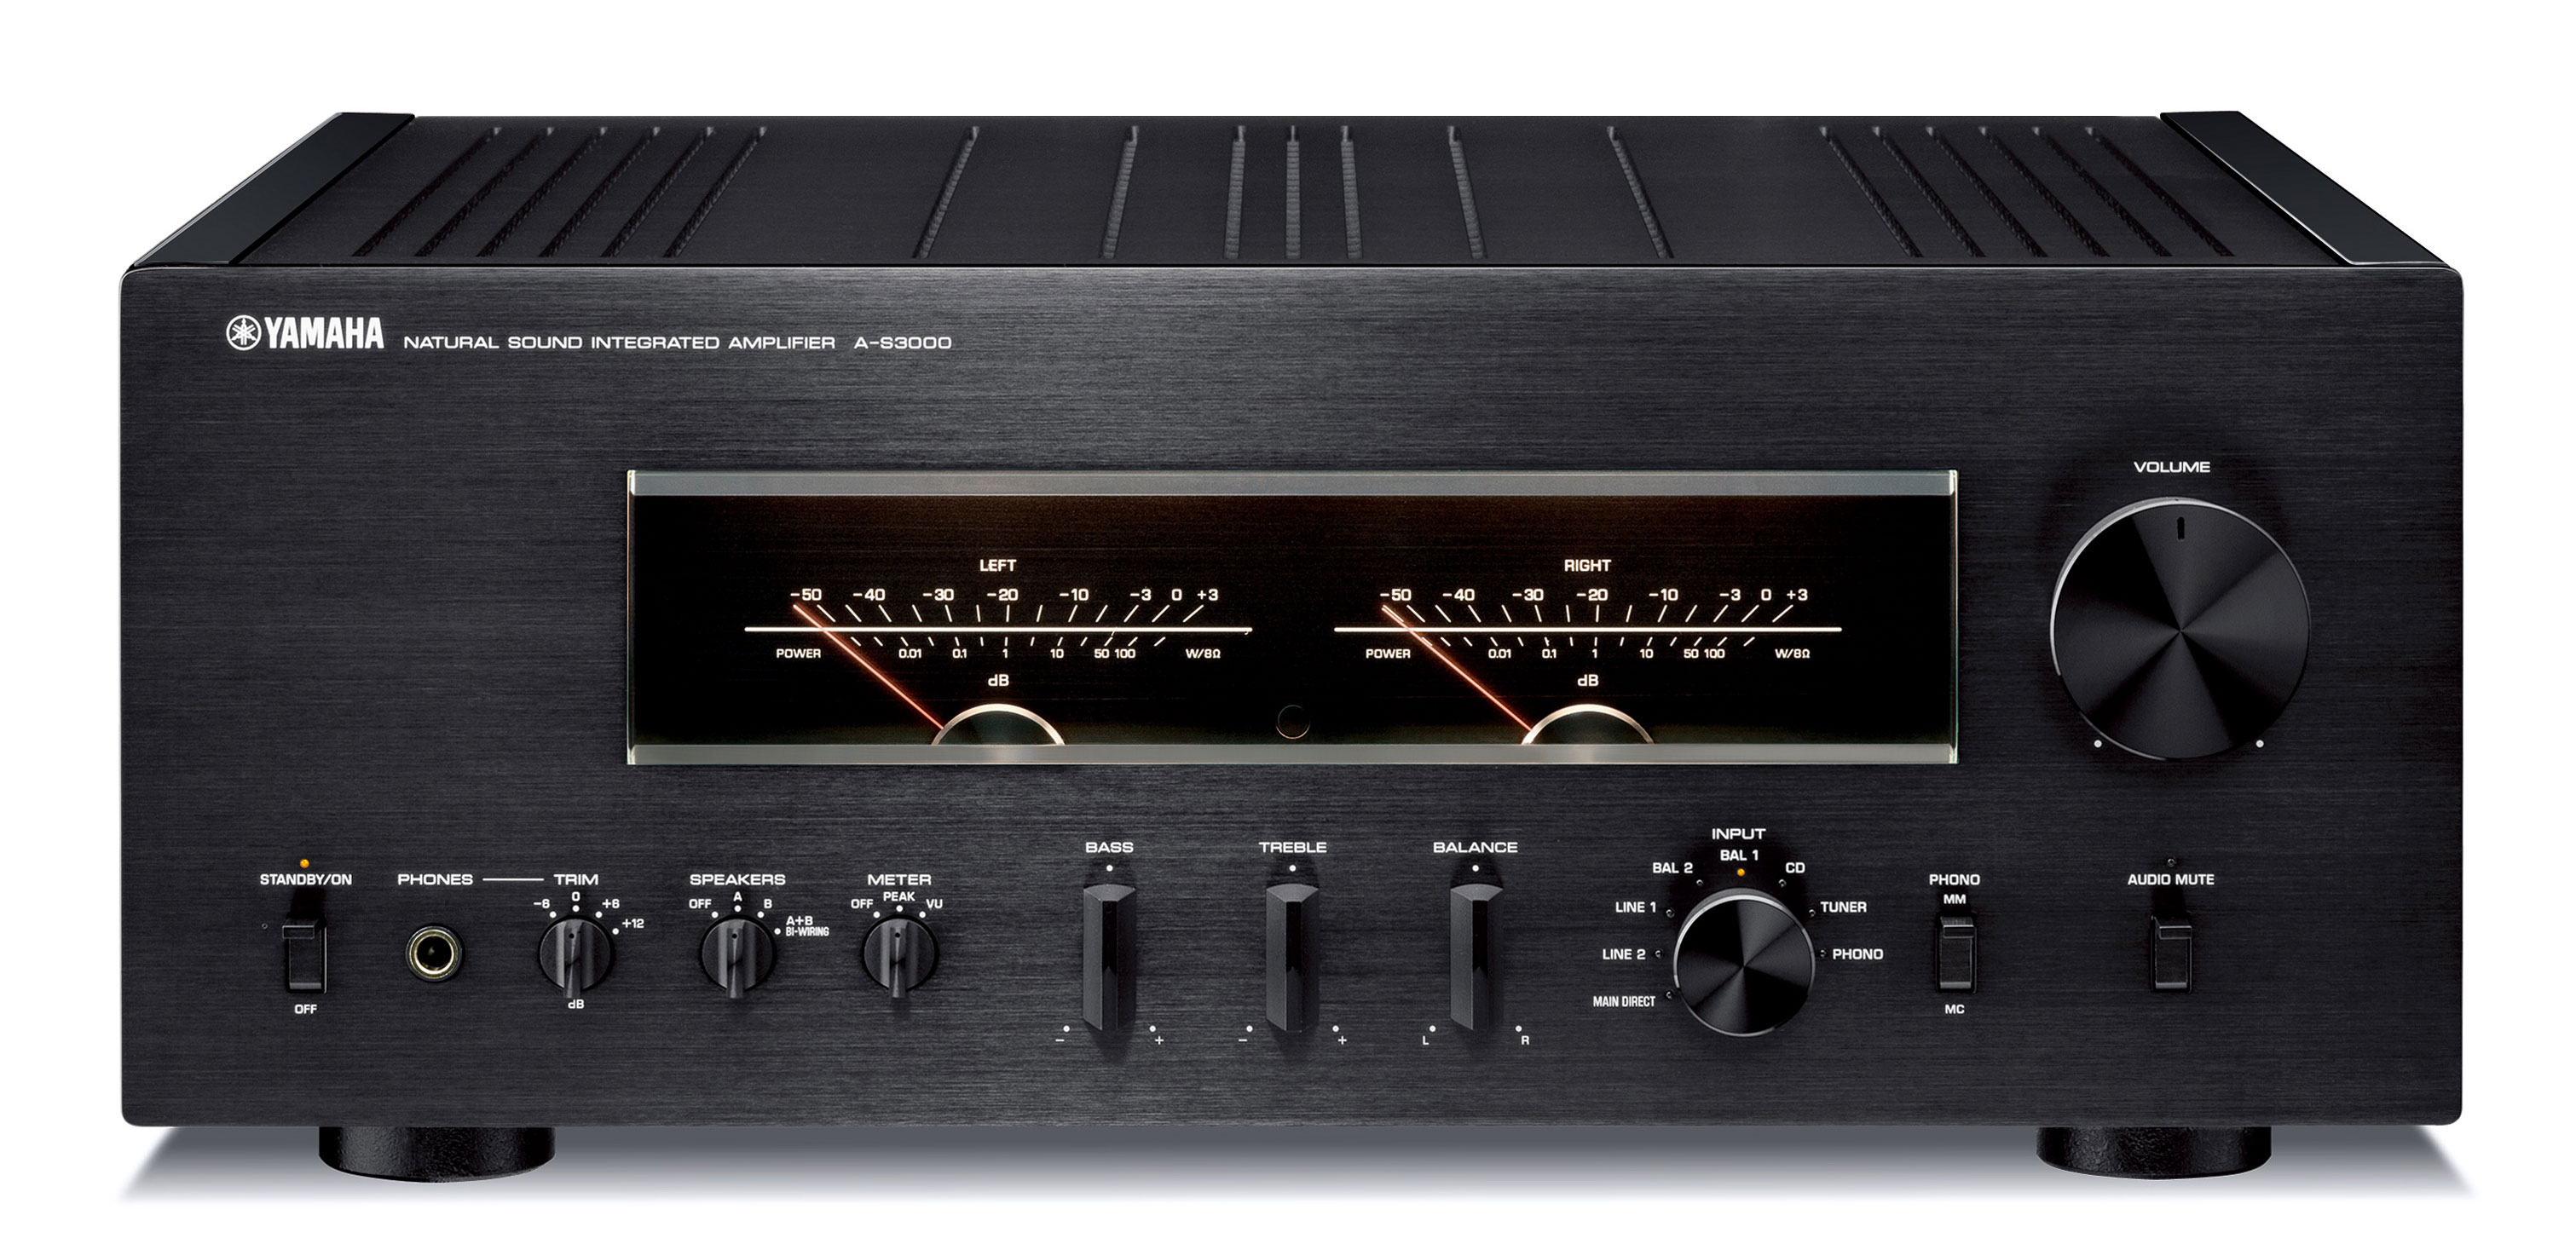
\includegraphics[width=\linewidth]{graphics/amplifier.jpg}
		\end{column}
	\end{columns}
\end{frame}

\note{Så problemet her er at jeg for nylig har købt mig en ny skabsfidus som nu huser min forstærker, en lille server og min router. 
Jeg kan ikke længere have skabet lukket, det bliver simpelthen for varmt, derfor ville jeg gerne have en temperatur styret blæser der kan sørge for at trække lidt af den varme luft ud af skabet.}

\begin{frame}
	\section{System Overview}
	\frametitle{System Overview}
	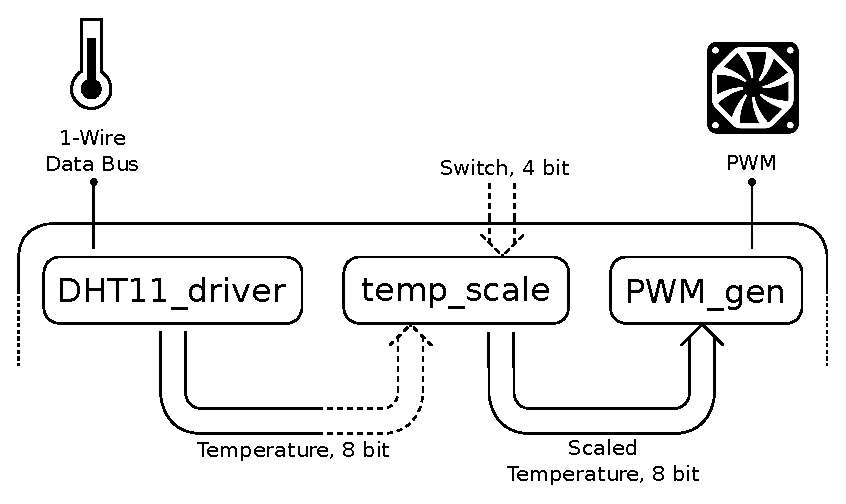
\includegraphics[width=\linewidth]{graphics/systemoverview.eps}
\end{frame}

\note{Så, det er værd at nævne at det ikke lykkedes mig at få projektet til at virke 100p.
Specifikt så havde jeg problemer med at aflæse datastrømmen korrekt.
Jeg valgte istedet at lave service virtualisation ved at simulere temperaturen med de switches der er tilgængelige på zyboen.
Desuden så er projektet lavet i ren VHDL.
Det vi ser på her er termometeret som vi kommunikerer med igennem en 1 wire bus som jeg kommer lidt mere ind på senere.
Den har jeg skrevet en driver til.
Udputtet fra driveren er naturligvis et tal, svarende til temperaturen.
For at oversætte temperaturen til pwm har jeg skrevet et modul der laver en skalering.
Til sidst her har vi en pwm generator som styrer hastigheden af blæseren, en ganske almindelig pc fan.}

\begin{frame}
	\section{DHT11}
	\frametitle{DHT11 Temperature Sensor}
	\centering
	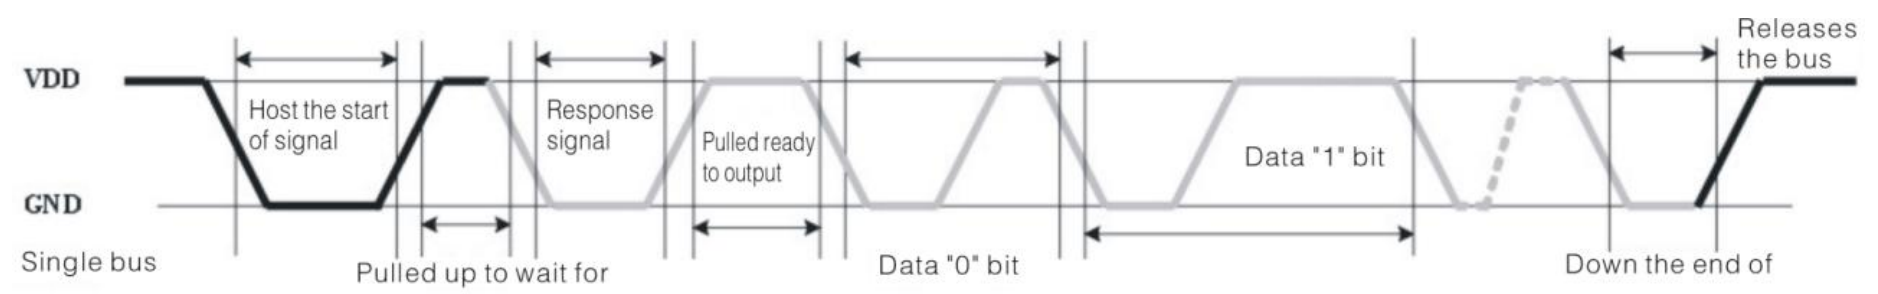
\includegraphics[width=\linewidth]{graphics/commcycle.png}
	\vfill
	\begin{columns}
		\begin{column}{.49\linewidth}
			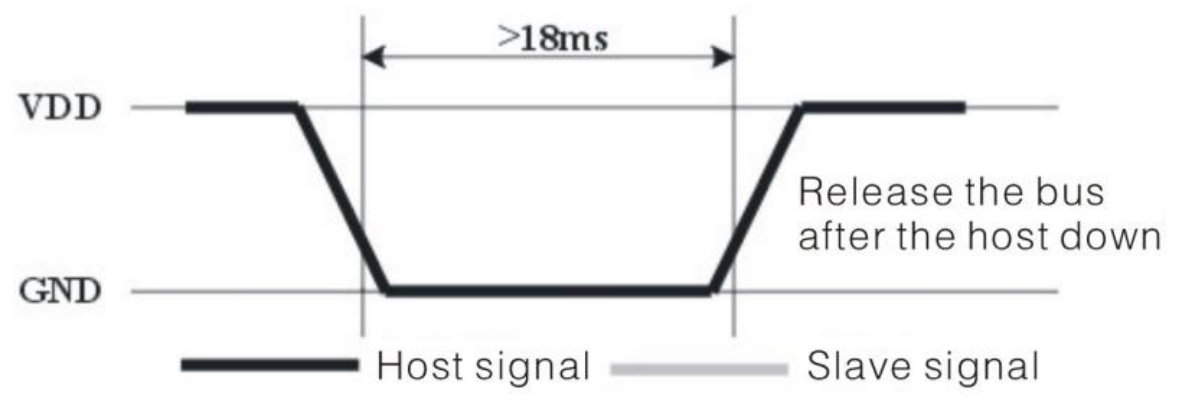
\includegraphics[width=\linewidth]{graphics/initcomm.png}
		\end{column}
		\begin{column}{.49\linewidth}
			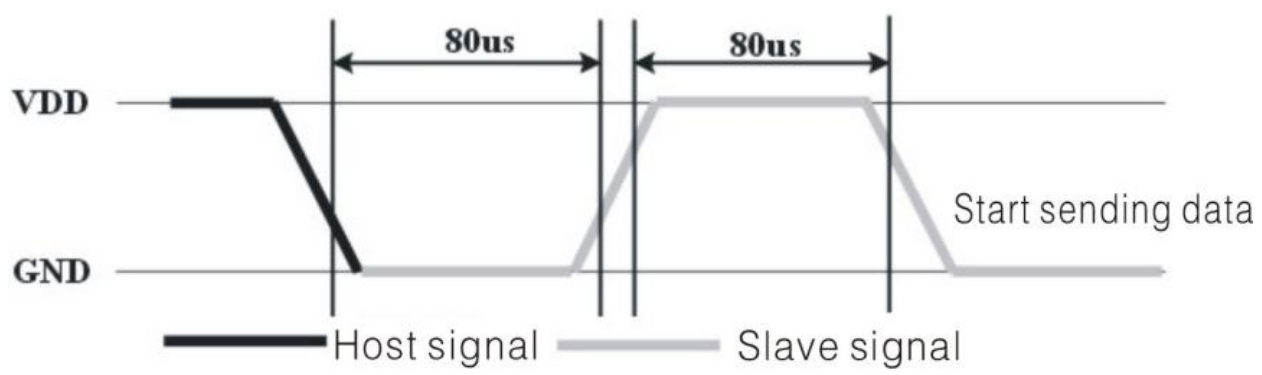
\includegraphics[width=\linewidth]{graphics/handshake.png}
		\end{column}
	\end{columns}
	\vfill
	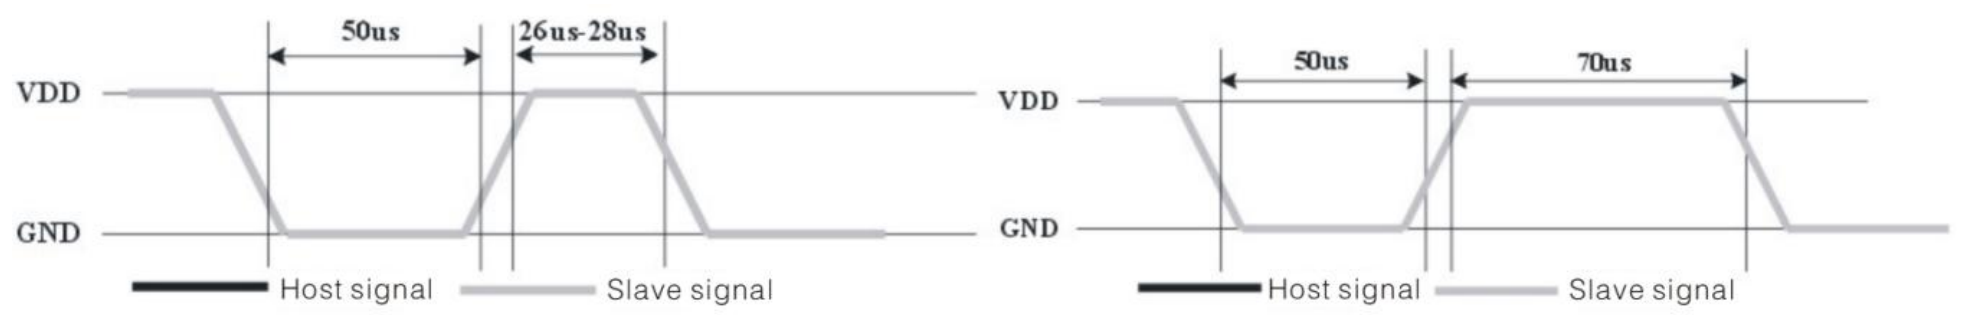
\includegraphics[width=\linewidth]{graphics/bit.png}
\end{frame}

\note{DHT11'eren er en kombineret temperatur og fugtigheds sensor.
Kommunikationen med den foregår, som jeg nævnte, over en 1-wire bus.
Vi kan her øverst se en hel kommunikations cycle.
Bussen har en pull up modstand til forsyningen, kommunikationen initialiseres ved at zybo'en trækker signalet lavt i 18ms og slipper så igen bussen.
Herefter vil sensoren køre et handshake ved at trække bussen ned i 80 us lade den være høj i 80 us hvorefter dataen sendes.
Hver data pakke består af 40 bit.
som vi kan se her forneden så er 0 lig en kort puls, dvs 25 ish us en lang puls er 1, 70 us ish.}

\begin{frame}
	\frametitle{DHT11 Driver}
	\centering
	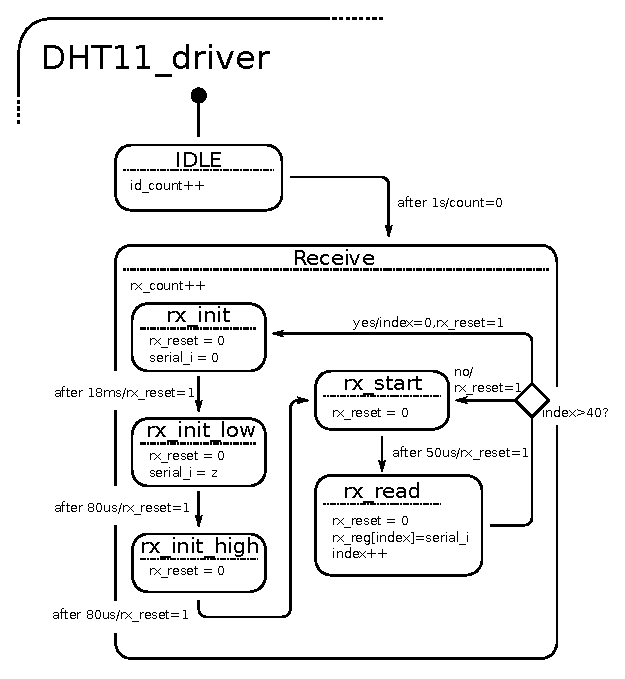
\includegraphics[height=.9\textheight]{graphics/dht11driver.eps}
\end{frame}

\begin{frame}
	\frametitle{DHT11 Driver - Output}
	\centering
	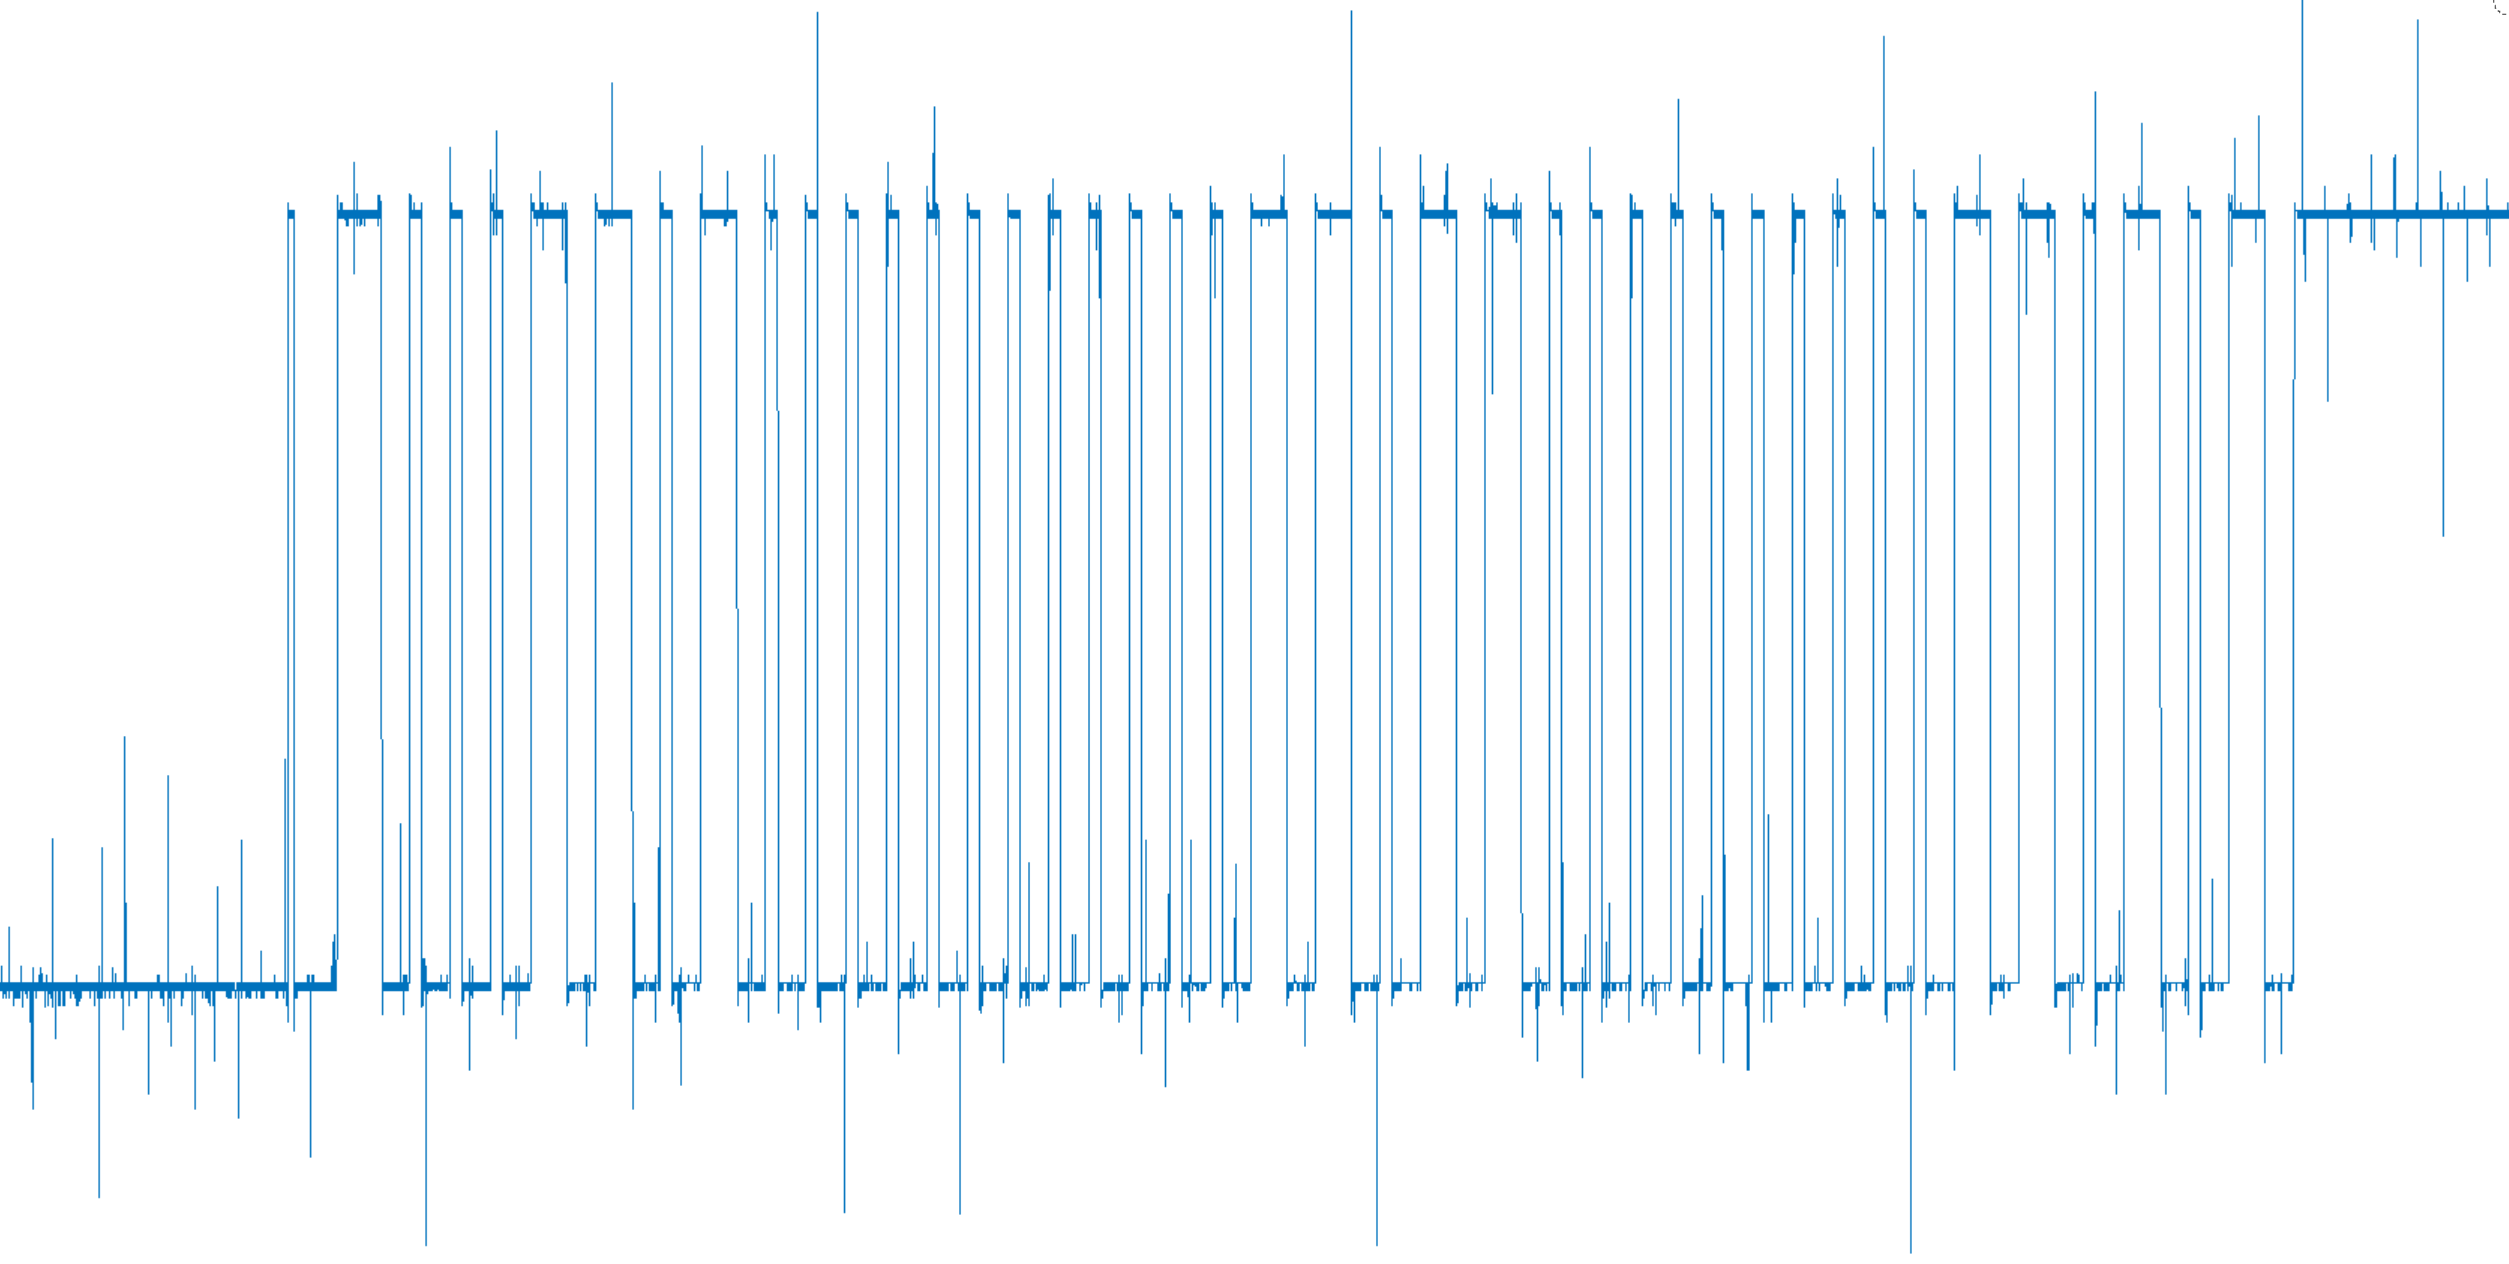
\includegraphics[width=1\textwidth]{graphics/temp.png}
\end{frame}

\begin{frame}
	\section{Temperature Scaling}
	\frametitle{Temperature Scaling}
	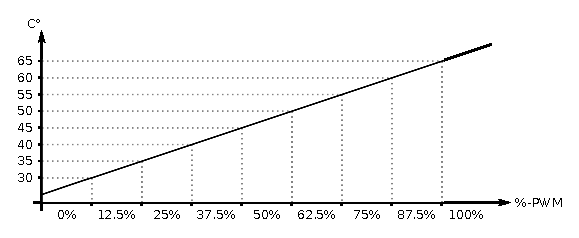
\includegraphics[width=\linewidth]{graphics/tempscale.eps}
\end{frame}

\begin{frame}
	\section{PWM Generation}
	\frametitle{PWM Generation}
	\begin{columns}
		\begin{column}{.49\linewidth}
			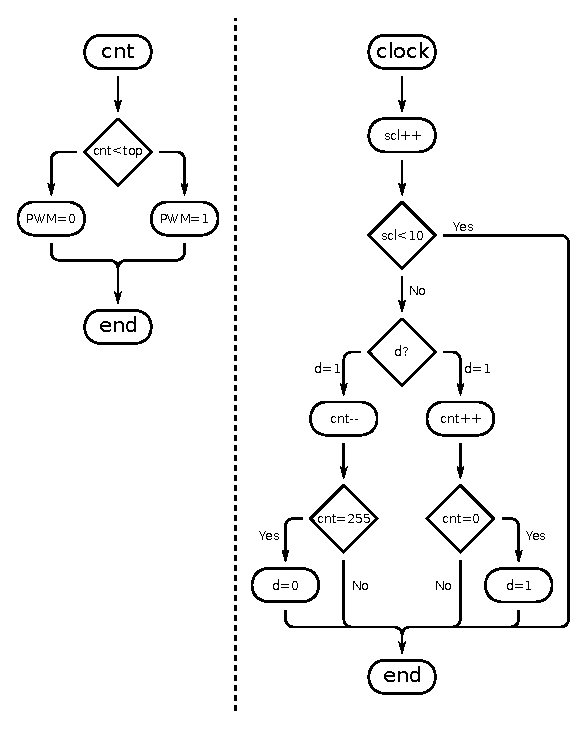
\includegraphics[width=\linewidth]{graphics/pwmgenerator.eps}
		\end{column}
		\begin{column}{.49\linewidth}
			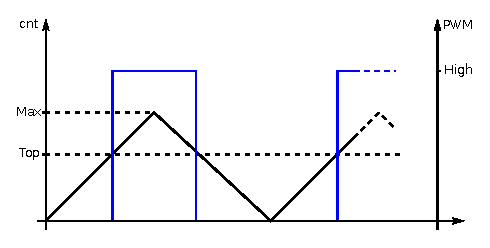
\includegraphics[width=\linewidth]{graphics/centeraligned.eps}
		\end{column}
	\end{columns}
\end{frame}

\end{document}